% article example for classicthesis.sty
\documentclass[10pt,a4paper]{article} % KOMA-Script article scrartcl
\usepackage{import}
\usepackage{xifthen}
\usepackage{pdfpages}
\usepackage{transparent}
\newcommand{\incfig}[1]{%
    \def\svgwidth{\columnwidth}
    \import{./figures/}{#1.pdf_tex}
}
\usepackage{lipsum}     %lorem ipsum text
\usepackage{titlesec}   %Section settings
\usepackage{titling}    %Title settings
\usepackage[margin=10em]{geometry}  %Adjusting margins
\usepackage{setspace}
\usepackage{listings}
\usepackage{amsmath}    %Display equations options
\usepackage{amssymb}    %More symbols
\usepackage{xcolor}     %Color settings
\usepackage{pagecolor}
\usepackage{mdframed}
\usepackage[spanish]{babel}
\usepackage[utf8]{inputenc}
\usepackage{longtable}
\usepackage{multicol}
\usepackage{graphicx}
\graphicspath{ {./Images/} }
\setlength{\columnsep}{1cm}

% ====| color de la pagina y del fondo |==== %
\pagecolor{white}
\color{black}



\begin{document}
    %========================{TITLE}====================%
    \title{{  10th lab  }}
    \author{{Rodrigo Castillo}}
    \date{\today}

    \maketitle


    %=======================NOTES GOES HERE===================%

    \section{Discover one free VPN that can be used to access to
    https://web.whatsapp.com/}
        there are many VPN services to access to whatsapp web, however if we're
        looking a vpn for using whatsapp, we want to use a vpn well ranked in
        privacy, thats why, according to the table, we are going to use
        AnonymousVPN

    \section{ From Intel product mentioned in slide 13, indicate which one of them is tactical,
        strategy and mixed intelligence product?}
        \textbf{Sophos 2020 Threat Report :}  strategic
        \\

        \textbf{THE WANNACRY RANSOMWARE:} mixed
        \\

        \textbf{EQUATION GROUP: QUESTIONS AND ANSWERS :} tactical
        \\

        \textbf{This Is Not a Test: APT41 Initiates Global Intrusion Campaign
        Using Multiple Exploits:} mixed




    \section{Research about the difference between TTP: Tactics, techniques and
    procedures?}

        \textbf{Tactics:}  makes reference to a global way to attack
        \\
        \textbf{Techniques:}  each tactics is divided in different ways to do it,
            each way to do it, its a technique
            \\
        \textbf{Procedure:}  its the way that techniques are implemented

    \section{What is the difference between an Indicator of compromise and of attack?}

        an indicator of an attack is an indicator that shows that an attack is
        incomming such a malicius hash detected. An indicator of compromise is
        an indicator that shows that an attack already succeed such a machine
        making things that is not supposed to do.

    \newpage
    \section{Review the indicators of compromise of Wannacry in
    https://otx.alienvault.com/ and find one atomic, computed and behavioral
    IoC.}
    \textbf{atomic:}
    \begin{figure}[h!]
        \centering
        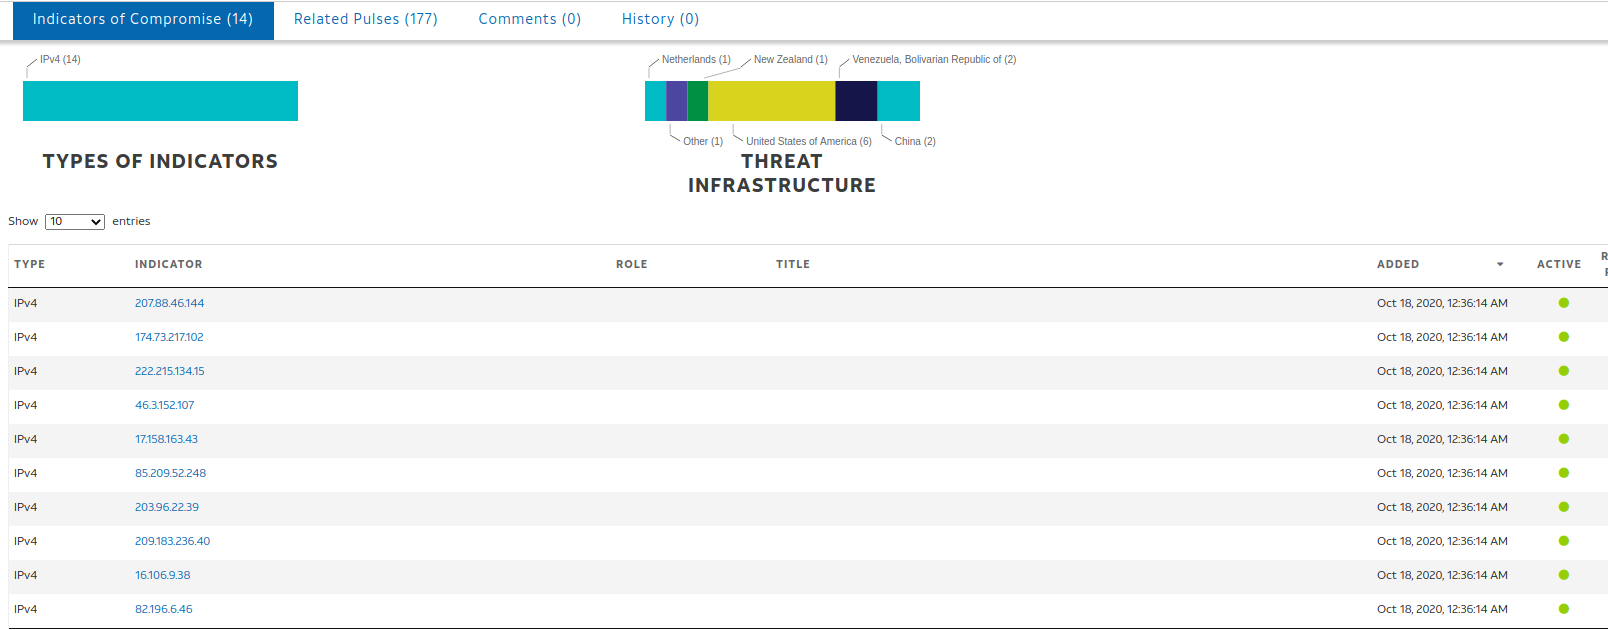
\includegraphics[width=1.0\linewidth]{bla.png}
        \caption{atomic}
        \label{atom}
    \end{figure}
    \textbf{computed:}

    \begin{figure}[h!]
        \centering
        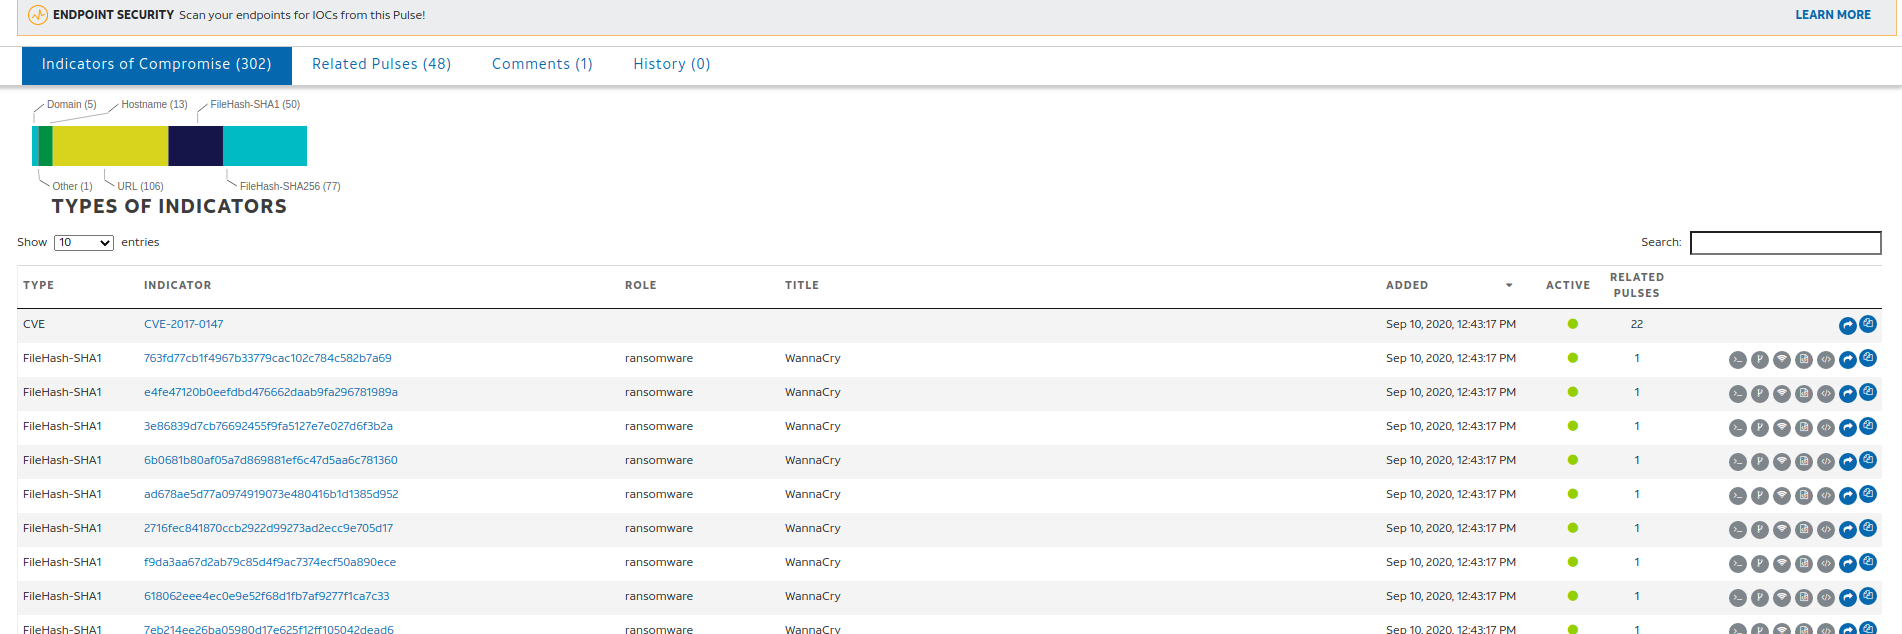
\includegraphics[width=1.0\linewidth]{bla2.png}
        \caption{nombre}
        \label{fig}
    \end{figure}


    \textbf{behavioral:}
    \begin{center}
        i didnt found none of those related to wannacry :(
    \end{center}























    %=======================NOTES ENDS HERE===================%

    % bib stuff
    \nocite{*}
    \addtocontents{toc}{{}}
    \addcontentsline{toc}{section}{\refname}
    \bibliographystyle{plain}
    \bibliography{../Bibliography}
\end{document}
